\documentclass[12pt]{article}
\usepackage[utf8]{inputenc}
\usepackage[T1]{fontenc}
\usepackage{geometry}
\usepackage{amsmath}
\usepackage{amssymb}
\usepackage{enumitem}
\usepackage{indentfirst}
\usepackage{xcolor}
\usepackage{fancyhdr}
\usepackage{graphicx}
\usepackage{float}

\geometry{a4paper, margin=1in}
\graphicspath{{img/}}

\pagestyle{fancy}
\fancyhf{} 
\fancyhead[L]{Informe: Simulación del Sistema de Reparación de Electrónica}
\renewcommand{\headrulewidth}{0.4pt} 
\setlength{\headheight}{15pt}

% Customize section headings
\renewcommand{\thesection}{\arabic{section}}
\renewcommand{\thesubsection}{\arabic{section}.\arabic{subsection}}
\renewcommand{\thesubsubsection}{\arabic{section}.\arabic{subsection}.\arabic{subsubsection}}

% Set paragraph indentation and spacing
\setlength{\parindent}{1em}
\setlength{\parskip}{0.5em}

% Custom list formatting
\setlist[itemize]{leftmargin=2em}
\setlist[enumerate]{leftmargin=2em}

\title{Informe: Simulación del Sistema de Reparación de Electrónica}
\author{José Ernesto Morales Lazo C-312}

\begin{document}

\maketitle 
\newpage

\section{Introducción}

\subsection{Descripción del Proyecto}
En este proyecto se simula un sistema de reparación de aparatos electrónicos en una empresa que presta servicios a minoristas de electrodomésticos en la región. La empresa recibe aparatos defectuosos y los clasifica según el tipo de reparación: general, especializada o almacén para regresarlo al fabricante. Además, los repara (si es necesario) y los prepara para su envío, ya sea al fabricante o de vuelta al cliente.

\subsection{Objetivos y Metas}
El objetivo principal es analizar el desempeño del sistema en términos de:
\begin{enumerate}
    \item Número promedio de aparatos en cada sección (clasificación, reparaciones generales, reparaciones por expertos y almacén).
    \item Tiempo promedio que un aparato pasa en cada sección, incluyendo espera y servicio.
    \item Tiempo total que un aparato permanece en la empresa desde su recepción hasta su empaque.
\end{enumerate}

\subsection{Sistema Específico a Simular y Variables de Interés}
El sistema consiste en una red de colas con cuatro tipos de servidores:
\begin{itemize}
    \item Clasificación: Inspección inicial para determinar el destino del aparato.
    \item Reparaciones Generales: Reparaciones básicas realizadas por tres técnicos.
    \item Reparaciones por Expertos: Reparaciones especializadas realizadas por cuatro expertos.
    \item Almacén: Preparación para envío, con dos muelles de embarque.
\end{itemize}
Las variables de interés incluyen:
\begin{itemize}
    \item Longitud promedio de las colas en cada nodo.
    \item Tiempos de espera y servicio por nodo.
    \item Tiempo total en el sistema.
    \item Utilización de los servidores en cada nodo.
    \item Distribución de aparatos por trayectorias posibles.
\end{itemize}

\subsection{Variables que Describen el Problema}
\begin{itemize}
    \item Tasa de llegada: 9 aparatos por hora (distribución de Poisson).
    \item Tiempos de servicio (distribuciones exponenciales):
    \begin{itemize}
        \item Clasificación: 6 minutos por aparato.
        \item Reparaciones generales: 35 minutos por aparato.
        \item Reparaciones por expertos: 65 minutos por aparato.
        \item Almacén: 12.5 minutos por aparato.
    \end{itemize}
    \item Probabilidades de redirección:
    \begin{itemize}
        \item Desde clasificación: 17\% al almacén, 57\% de los restantes (47.31\% del total) a reparaciones generales, 43\% de los restantes (35.69\% del total) a expertos.
        \item Desde reparaciones generales: 5\% regresa a clasificación, 95\% al almacén.
    \end{itemize}
\end{itemize}

\section{Detalles de Implementación}
La simulación se implementó utilizando un enfoque de simulación de eventos discretos. Los pasos seguidos fueron:
\begin{enumerate}
    \item Definición de la Clase \texttt{ElectronicsRepair}:
    \begin{enumerate}
        \item Se creó una clase que encapsula el estado del sistema, incluyendo colas, servidores, tiempos de eventos y estadísticas.
        \item Se inicializaron parámetros como la tasa de llegada, funciones para generar tiempos de servicio (exponenciales) y duración de la simulación (24 horas).
    \end{enumerate}
    \item Modelado de Eventos:
    \begin{enumerate}
        \item Se definieron cinco tipos de eventos: llegada de un aparato, fin de clasificación, fin de reparación general, fin de reparación por expertos y fin de procesamiento en almacén.
        \item Cada evento actualiza el estado del sistema (colas, servidores, tiempos) y genera nuevos eventos según las probabilidades de redirección.
    \end{enumerate}
    \item Gestión de Colas y Servidores:
    \begin{enumerate}
        \item Clasificación: Una cola FIFO con un servidor.
        \item Reparaciones generales: Tres colas (una por servidor) con asignación aleatoria.
        \item Reparaciones por expertos: Cuatro colas con asignación aleatoria.
        \item Almacén: Dos colas con asignación aleatoria.
        \item Se registran los tiempos de espera y servicio para cada aparato.
    \end{enumerate}
    \item Recolección de Estadísticas:
    \begin{enumerate}
        \item Se registraron longitudes de cola en cada evento, tiempos de inicio y fin por nodo, trayectorias de los aparatos y utilización de servidores.
        \item Se calcularon promedios ponderados por tiempo para las longitudes de cola y estadísticas de tiempos (espera, servicio, sistema).
    \end{enumerate}
    \item Ejecución de la Simulación:
    \begin{enumerate}
        \item La simulación se llevó a cabo, generando eventos hasta que la cola de eventos se vació o se alcanzó el tiempo límite.
    \end{enumerate}
\end{enumerate}

\section{Resultados y Experimentos}

\subsection{Hallazgos de la Simulación}
La simulación procesó 219 aparatos, con los siguientes resultados:
\begin{itemize}
    \item Un promedio de 6 aparatos en cola de clasificación con tiempo de espera de 54.86 minutos
    \item Un promedio de 8, 3, 4 aparatos en cola de reparaciones generales (54.86 minutos de espera), expertos (80.43 minutos de espera) y almacén (32.91 minutos de espera) respectivamente.
    \begin{figure}[H]
        \centering
        \begin{minipage}{0.45\textwidth}
            \centering
            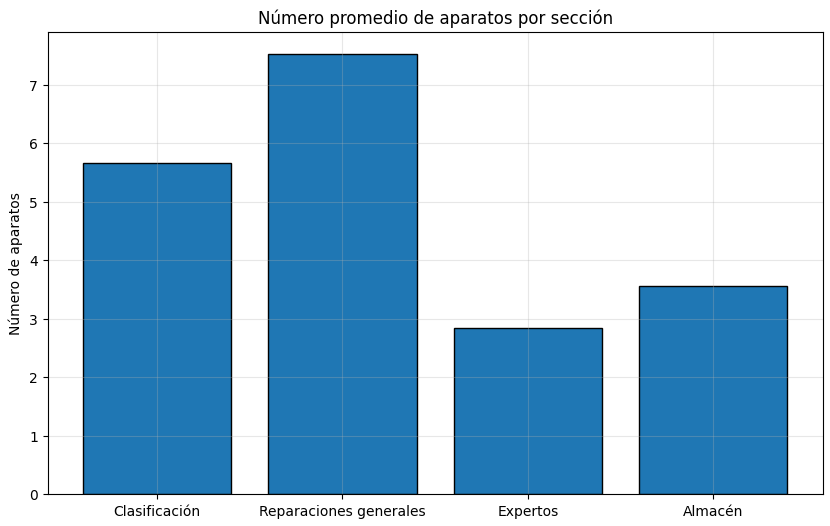
\includegraphics[width=\textwidth]{appliences_queue.png}
            \caption{Cantidad promedio de aparatos por cola}
            \label{fig: Cantidad promedio de aparatos por cola}
        \end{minipage}
        \hfill
        \begin{minipage}{0.45\textwidth}
            \centering
            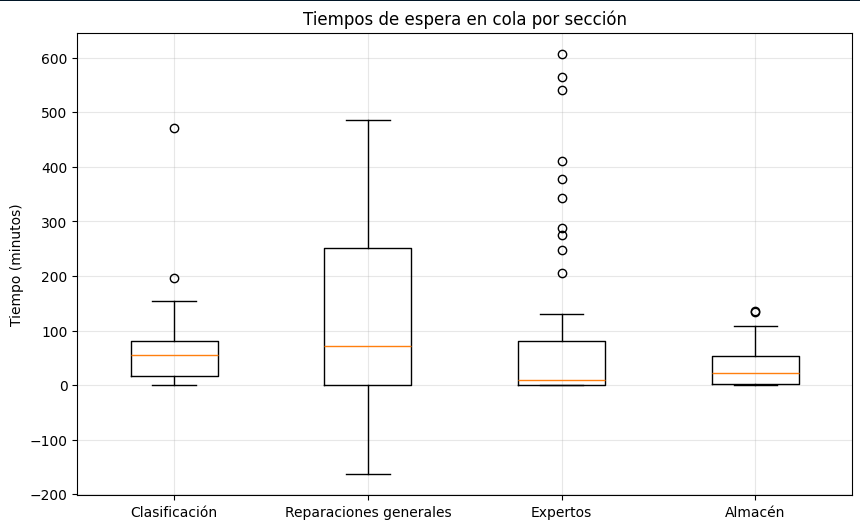
\includegraphics[width=\textwidth]{queue_times.png}
            \caption{Tiempos en colas}
            \label{fig: Tiempo en cada cola}
        \end{minipage}
    \end{figure}
    \item El tiempo promedio de servicio es 6.75 minutos en clasificación, 34.15 minutos en reparaciones generales, 63.64 con los expertos y 13.12 minutos en el almacén
    \begin{figure}[H]
        \centering
        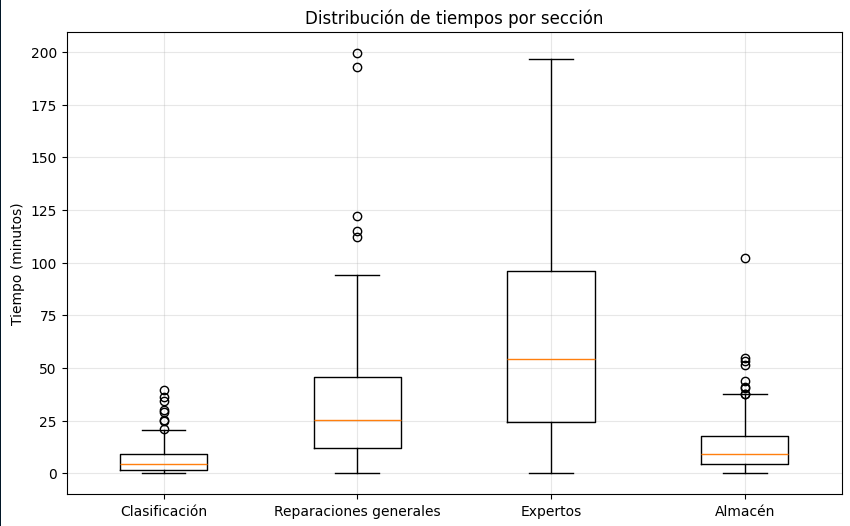
\includegraphics[width=0.8\textwidth]{section_times.png}
        \caption{Tiempo que demora un aparato en cada sección}
        \label{fig: Tiempo que demora un aparato en cada sección}
    \end{figure}
    \item Las trayectorias seguidas fueron:
    \begin{itemize}
        \item Clasificación a almacén: 40 aparatos (18.26\%).
        \item Clasificación a reparaciones generales a almacén: 103 aparatos (47.03\%).
        \item Clasificación a expertos a almacén: 70 aparatos (31.96\%).
        \item Clasificación a reparaciones generales a clasificación a almacén: 3 aparatos (1.37\%).
        \item Clasificación a reparaciones generales a clasificación a expertos: 0 aparatos (0\%).
    \end{itemize}
    \begin{figure}[H]
        \centering
        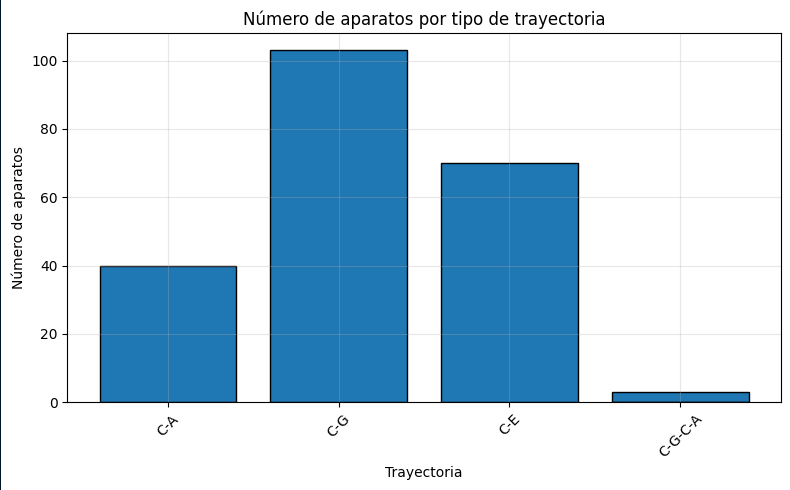
\includegraphics[width=0.8\textwidth]{trajectories.png}
        \caption{Cantidad de aparatos por trayectoria}
        \label{fig: Cantidad de aparatos por trayectoria}
    \end{figure}
    \item El servidor de clasificaciones estuvo ocupado el 73.18\% del tiempo.
    \item Los servidores de reparaciones generales reciben entre 30 y 45 aparatos aproximadamente con un total entre los tres de 108 aparatos, mientras que los servidores de expertos reciben entre 10 y 25 aparatos con un total de 70.
    \item Los muelles reciben todos los aparatos, atendiendo cada uno alrededor de 110 aparatos.
    \item Los servidores de reparaciones generales se mantienen ocupados un promedio de 60.93\% de tiempo variando cada uno entre el 45\% y 85\%.
    \item En el caso de expertos el tiempo promedio ocupado es 55.63\% distribuidos entre un 35\% y 80\% por servidor.
    \item En los muelles se distribuye el tiempo en que están ocupados entre un 65\% y 75\%.
    \begin{figure}[H]
        \centering
        \begin{minipage}{0.45\textwidth}
            \centering
            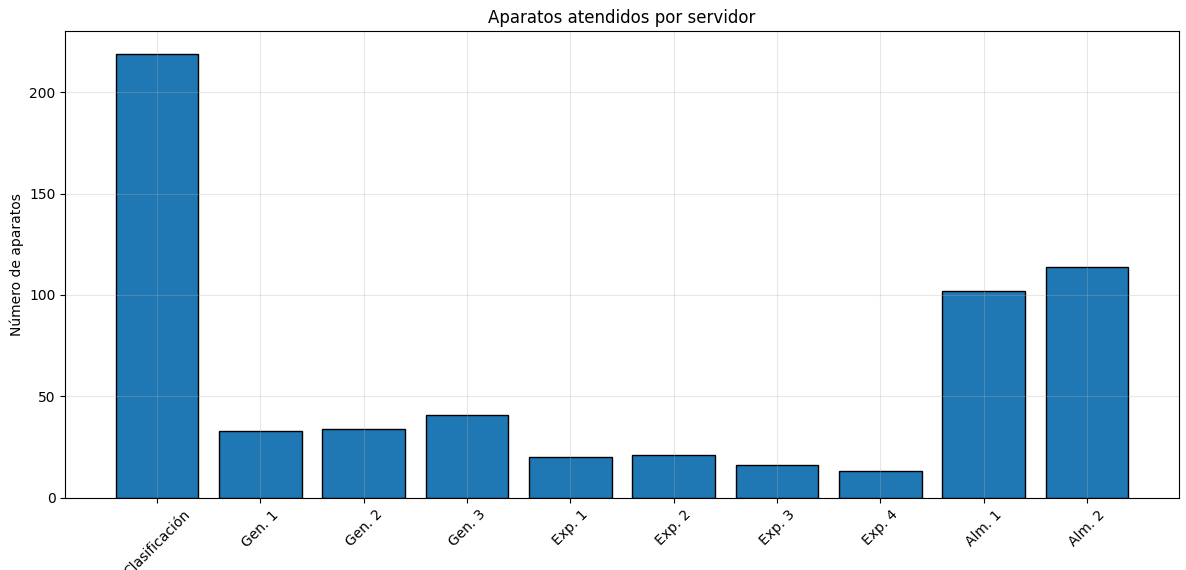
\includegraphics[width=\textwidth]{server_appliences.png}
            \caption{Cantidad de aparatos por servidor}
            \label{fig: Cantidad de aparatos por servidor}
        \end{minipage}
        \hfill
        \begin{minipage}{0.45\textwidth}
            \centering
            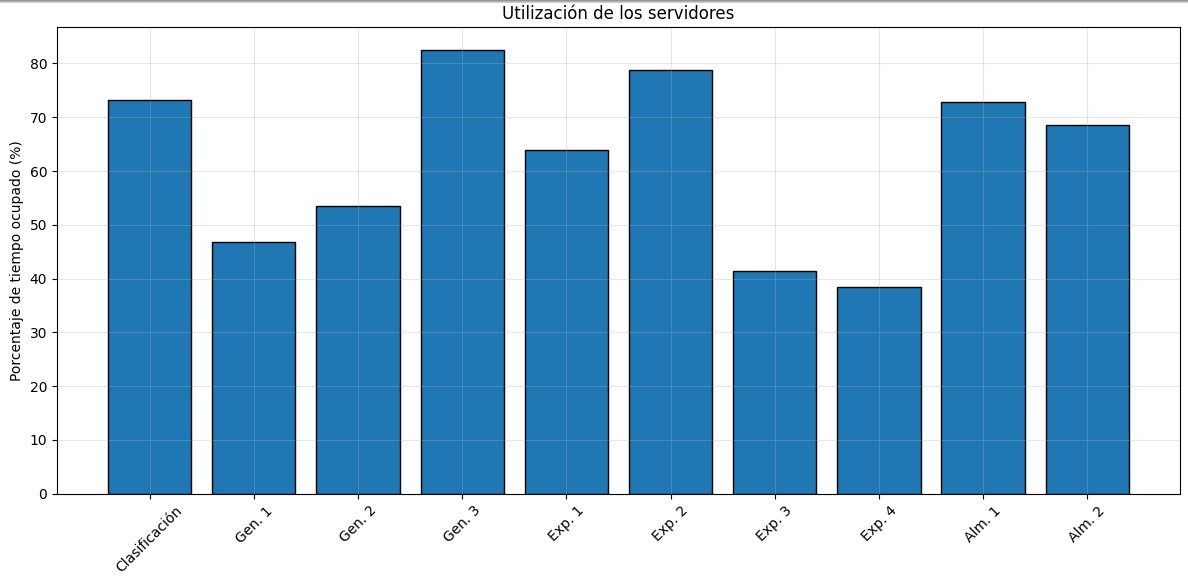
\includegraphics[width=\textwidth]{server_utilization.png}
            \caption{Porciento de tiempo que estuvo ocupado cada servidor}
            \label{fig: Porciento de tiempo que estuvo ocupado cada servidor}
        \end{minipage}
    \end{figure}
    \item 3 aparatos reingresaron a clasificación desde reparaciones generales (tasa de reingreso: 1.39\%).
    \begin{figure}[H]
        \centering
        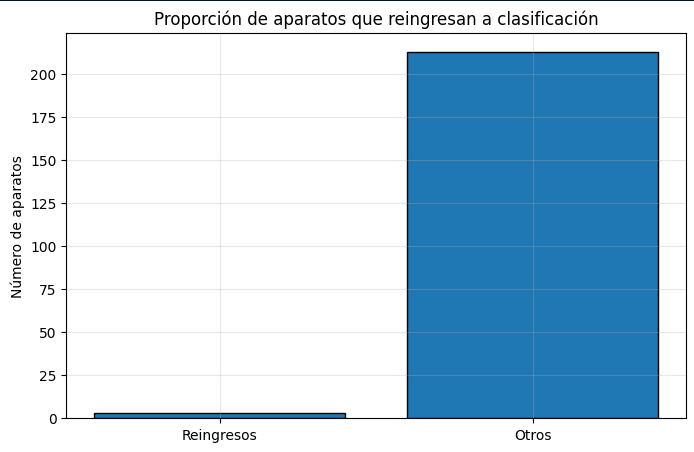
\includegraphics[width=0.8\textwidth]{clasification.png}
        \caption{Redirección a clasificaciones comparado con otras trayectorias}
        \label{fig: Redirección a clasificaciones comparado con otras trayectorias}
    \end{figure}
    \item El tiempo promedio de un aparato en el sistema es de 238.62 minutos (aproximadamente 4 horas).
    \begin{figure}[H]
        \centering
        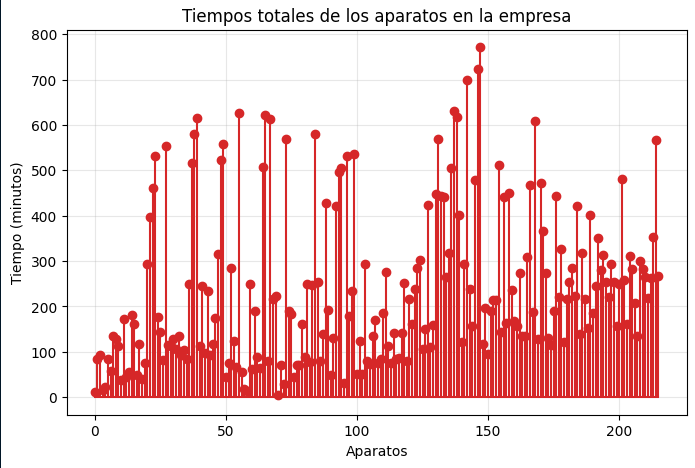
\includegraphics[width=0.8\textwidth]{time.png}
        \caption{Tiempo en el sistema de cada aparato}
        \label{fig: Tiempo en el sistema de cada aparato}
    \end{figure}
\end{itemize}

\subsection{Interpretación de los Resultados}
\begin{itemize}
    \item Clasificación: La alta utilización (73.18\%) y el número promedio de aparatos (5.67) indican una carga significativa en el único servidor, con tiempos de espera considerables (54.86 minutos). Esto sugiere que posiblemente limite el flujo de las reparaciones.
    \item Reparaciones Generales: El tiempo de espera en cola (136.48 minutos) es el más alto, a pesar de tener tres servidores.
    \item Expertos: La menor longitud de cola (2.84) y tiempos de espera razonables (80.43 minutos) reflejan una buena capacidad.
    \item Almacén: La longitud de cola (3.55) y el tiempo de espera (32.91 minutos) son moderados, con una utilización equilibrada (\textasciitilde 70\%), lo que indica un desempeño adecuado.
    \item Tiempo Total: Los 238.62 minutos reflejan la complejidad de las trayectorias, especialmente para aparatos que pasan por reparaciones generales o expertos, donde los tiempos de espera dominan.
\end{itemize}

\subsection{Hipótesis Extraídas}
\begin{enumerate}
    \item H1: El nodo de clasificación limita el flujo debido a su alta utilización y tiempos de espera prolongados.
    \item H2: El tiempo total en el sistema está dominado por los tiempos de espera en reparaciones generales y expertos, más que por los tiempos de servicio.
\end{enumerate}

\subsection{Experimentos Realizados}
Para validar las hipótesis, se realizaron experimentos adicionales:
\begin{itemize}
    \item Experimento 1: Incrementar los servidores de clasificación de 1 a 2 y que trabajan los dos servidores en paralelo.
    \begin{itemize}
        \item Resultado: La cola promedio en clasificación cayó a 0 aparatos y el tiempo de espera a 4.23 minutos.
        \item Conclusión: H1 confirmada; más servidores en clasificación mejoran significativamente el desempeño.
    \end{itemize}
    \item Experimento 2: Agregar un servidor a reparaciones generales y otro a expertos.
    \begin{itemize}
        \item Resultado: El tiempo en el sistema se redujo a 167.46 minutos (aproximadamente 3 horas).
        \item Conclusión: H2 confirmada; más servidores en reparaciones generales y en expertos disminuyen significativamente el tiempo en la empresa.
    \end{itemize}
\end{itemize}

\subsection{Análisis Estadístico}
Las variables de interés (longitudes de cola, tiempos de espera, tiempos de servicio, tiempo total en el sistema, utilización, trayectorias) son críticas para evaluar el desempeño del sistema, pero su estimación precisa requiere un análisis estadístico por las siguientes razones:
\begin{itemize}
    \item Variabilidad Inherente: Las distribuciones exponenciales de llegadas y servicios introducen alta variabilidad.
    \item Tamaño Finito de la Muestra: Una sola corrida de 24 horas (219 aparatos) no garantiza que las estimaciones representen el comportamiento a largo plazo, especialmente para eventos raros como reingresos (1.39\% vs. 5\% esperado).
    \item Variables Clave:
    \begin{itemize}
        \item Longitudes de cola: Necesitamos intervalos de confianza para confirmar si la reducción en clasificación (\textasciitilde 0.36 aparatos) es consistente.
        \item Tiempos de espera: La variabilidad en reparaciones generales (136.48 minutos) requiere análisis para determinar si es un problema estructural o un artefacto de la simulación.
        \item Tiempo total: Es crítico para la satisfacción del cliente, y su estimación (238.62 minutos) debe validarse para asegurar que refleja el promedio real.
    \end{itemize}
\end{itemize}

\subsection{Análisis de Parada}
La simulación se detuvo tras 24 horas, procesando 219 aparatos. Aunque esto proporciona una buena muestra, la alta variabilidad en los tiempos de espera sugiere que una simulación más larga o múltiples corridas podrían estabilizar las estimaciones.

\section{Modelo Matemático}

\subsection{Descripción del Modelo}
El sistema se modela como una red de colas con cuatro nodos:
\begin{itemize}
    \item Clasificación: Cola M/M/1 con un servidor.
    \item Reparaciones Generales: Cola M/M/3 con tres servidores.
    \item Reparaciones por Expertos: Cola M/M/4 con cuatro servidores.
    \item Almacén: Cola M/M/2 con dos servidores.
\end{itemize}
Las llegadas siguen una distribución de Poisson, y los tiempos de servicio son exponenciales. Las tasas de llegada efectivas se calculan considerando las redirecciones:
\begin{itemize}
    \item Clasificación: $\lambda_c = \lambda + 0.05 \cdot \lambda_g$, donde $\lambda = 9$/hora.
    \item Reparaciones Generales: $\lambda_g = 0.4731 \cdot \lambda_c$.
    \item Expertos: $\lambda_e = 0.3569 \cdot \lambda_c$.
    \item Almacén: $\lambda_w = 0.17 \cdot \lambda_c + 0.95 \cdot \lambda_g + \lambda_e$.
\end{itemize}
Resolviendo:
\begin{itemize}
    \item $\lambda_c \approx 9.47$ aparatos/hora ($9 + 0.05 \cdot 4.48$).
    \item $\lambda_g \approx 4.48$ aparatos/hora ($0.4731 \cdot 9.47$).
    \item $\lambda_e \approx 3.38$ aparatos/hora ($0.3569 \cdot 9.47$).
    \item $\lambda_w \approx 9.11$ aparatos/hora ($0.17 \cdot 9.47 + 0.95 \cdot 4.48 + 3.38$).
\end{itemize}

\subsection{Cálculos Teóricos}

\begin{itemize}
    \item Clasificación (M/M/1):
    \begin{itemize}
        \item $\mu_c = 60/6 = 10$/hora.
        \item $\rho_c = 9.47/10 = 0.947$.
        \item $L_q = \rho_c^2/(1 - \rho_c) \approx 17.09$ aparatos.
        \item $L = L_q + \rho_c \approx 18.04$ aparatos.
        \item $W_q = L_q/\lambda_c \approx 1.80$ horas $\approx 108$ minutos.
        \item $W = W_q + 1/\mu_c \approx 108 + 6 \approx 114$ minutos.
    \end{itemize}
    \item Reparaciones Generales (M/M/3):
    \begin{itemize}
        \item $\mu_g = 60/35 \approx 1.714$/hora.
        \item $\rho_g = 4.48/(3 \cdot 1.714) \approx 0.872$.
        \item $a = \lambda_g/\mu_g \approx 2.615$.
        \item $P_0 \approx 0.023$ (calculado numéricamente).
        \item $L_q \approx 10.12$ aparatos.
        \item $L = L_q + a \approx 12.73$ aparatos.
        \item $W_q = L_q/\lambda_g \approx 2.26$ horas $\approx 135.6$ minutos.
        \item $W = W_q + 1/\mu_g \approx 135.6 + 35 \approx 170.6$ minutos.
    \end{itemize}
    \item Expertos (M/M/4):
    \begin{itemize}
        \item $\mu_e = 60/65 \approx 0.923$/hora.
        \item $\rho_e = 3.38/(4 \cdot 0.923) \approx 0.916$.
        \item $a = \lambda_e/\mu_e \approx 3.66$.
        \item $P_0 \approx 0.012$.
        \item $L_q \approx 4.80$ aparatos.
        \item $L = L_q + a \approx 8.46$ aparatos.
        \item $W_q = L_q/\lambda_e \approx 1.42$ horas $\approx 85.2$ minutos.
        \item $W = W_q + 1/\mu_e \approx 85.2 + 65 \approx 150.2$ minutos.
    \end{itemize}
    \item Almacén (M/M/2):
    \begin{itemize}
        \item $\mu_w = 60/12.5 = 4.8$/hora.
        \item $\rho_w = 9.11/(2 \cdot 4.8) \approx 0.948$.
        \item $a = \lambda_w/\mu_w \approx 1.898$.
        \item $P_0 \approx 0.159$.
        \item $L_q \approx 4.62$ aparatos.
        \item $L = L_q + a \approx 6.52$ aparatos.
        \item $W_q = L_q/\lambda_w \approx 0.51$ horas $\approx 30.6$ minutos.
        \item $W = W_q + 1/\mu_w \approx 30.6 + 12.5 \approx 43.1$ minutos.
    \end{itemize}
\end{itemize}

\subsection{Supuestos y Restricciones}
\begin{itemize}
    \item Distribuciones exponenciales: Llegadas y servicios son exponenciales, asumiendo procesos sin memoria.
    \item Capacidad infinita: No hay límite en las colas.
    \item Estado estacionario: El sistema alcanza un equilibrio a largo plazo.
    \item Independencia: Las decisiones de redirección son independientes.
    \item Tiempos de transición negligible: No se consideran demoras adicionales entre nodos.
\end{itemize}

\subsection{Comparación con Resultados Experimentales}
\begin{itemize}
    \item Clasificación:
    \begin{itemize}
        \item Teórico: $L_q \approx 17.09$, $W_q \approx 108$ minutos, $L \approx 18.04$, $W \approx 114$ minutos.
        \item Simulación: $L_q \approx 5.67$, $W_q \approx 54.86$ minutos, $W \approx 61.61$ minutos.
        \item Análisis: La simulación reporta valores significativamente menores, posiblemente debido a un tiempo de simulación finito (24 horas) que no captura el estado estacionario completo. La alta utilización teórica (94.7\%) sugiere saturación, pero la simulación indica una carga más manejable (73.18\%).
    \end{itemize}
    \item Reparaciones Generales:
    \begin{itemize}
        \item Teórico: $L_q \approx 10.12$, $W_q \approx 135.6$ minutos, $L \approx 12.73$, $W \approx 170.6$ minutos.
        \item Simulación: $L_q \approx 7.52$, $W_q \approx 136.48$ minutos, $W \approx 170.63$ minutos.
        \item Análisis: Los tiempos de espera y totales son muy cercanos, validando el modelo para este nodo. La longitud de cola simulada es ligeramente menor, posiblemente por efectos aleatorios o una distribución desigual entre servidores.
    \end{itemize}
    \item Expertos:
    \begin{itemize}
        \item Teórico: $L_q \approx 4.80$, $W_q \approx 85.2$ minutos, $L \approx 8.46$, $W \approx 150.2$ minutos.
        \item Simulación: $L_q \approx 2.84$, $W_q \approx 80.43$ minutos, $W \approx 144.07$ minutos.
        \item Análisis: Los valores son cercanos, con una ligera subestimación en la simulación, probablemente por la variabilidad en la asignación de tareas entre expertos.
    \end{itemize}
    \item Almacén:
    \begin{itemize}
        \item Teórico: $L_q \approx 4.62$, $W_q \approx 30.6$ minutos, $L \approx 6.52$, $W \approx 43.1$ minutos.
        \item Simulación: $L_q \approx 3.55$, $W_q \approx 32.91$ minutos, $W \approx 46.03$ minutos.
        \item Análisis: Los resultados son consistentes, con diferencias menores atribuibles a fluctuaciones aleatorias.
    \end{itemize}
    \item Tiempo Total en el Sistema:
    \begin{itemize}
        \item Teórico: Calculado ponderando trayectorias:
        \begin{itemize}
            \item Clasificación a almacén (\textasciitilde 17\%): $W \approx 6 + 12.5 = 18.5$ minutos.
            \item Clasificación a generales a almacén (\textasciitilde 44.99\%): $W \approx 6 + 170.6 + 12.5 \approx 189.1$ minutos.
            \item Clasificación a expertos a almacén (\textasciitilde 35.69\%): $W \approx 6 + 150.2 + 12.5 \approx 168.7$ minutos.
            \item Otros (\textasciitilde 2.32\%): Incluyen reingresos, estimado en \textasciitilde 200 minutos.
            \item $W_s \approx (0.17 \cdot 18.5) + (0.4499 \cdot 189.1) + (0.3569 \cdot 168.7) + (0.0232 \cdot 200) \approx 152.9$ minutos.
        \end{itemize}
        \item Simulación: $W_s \approx 238.62$ minutos.
        \item Análisis: La discrepancia (\textasciitilde 56\%) se debe principalmente a los tiempos de espera simulados más altos, especialmente en clasificación y reparaciones generales, que reflejan dinámicas no capturadas por el modelo teórico estacionario.
    \end{itemize}
\end{itemize}

\section{Conclusiones}
La simulación del sistema de reparación de electrónica proporciona una visión detallada del desempeño operativo:
\begin{itemize}
    \item Limitaciones del flujo: Clasificación y reparaciones generales son las secciones más congestionadas, con tiempos de espera prolongados (54.86 y 136.48 minutos, respectivamente) y longitudes de cola significativas (5.67 y 7.52 aparatos).
    \item Eficiencia: La sección de expertos y el almacén operan con mayor fluidez, aunque la utilización desigual en expertos sugiere oportunidades de optimización.
    \item Tiempo Total: Los 238.62 minutos en el sistema indican que los aparatos, especialmente los que requieren reparaciones, enfrentan demoras considerables debido a los tiempos de espera.
    \item Modelo vs. Realidad: El modelo matemático subestima los tiempos de espera en clasificación y sobreestima las longitudes de cola. Sin embargo, los resultados experimentales son útiles para identificar cuellos de botella y proponer mejoras.
\end{itemize}

\end{document}